\documentclass[12pt]{article}
\usepackage[a4paper, margin=.30in]{geometry}
\usepackage{graphicx ,
            wrapfig,
            xcolor, 
            enumerate,
            amsmath,fontenc
            }

\newcommand\headerMe[2]{\noindent{}#1\hfill#2}
\renewcommand{\thesection}{\Roman{section}}

\title{Leçon N 6 : Le mouvement}
\author{Zakaria HAOUZAN}
\date{\today}

\begin{document}
% headers --------------
\headerMe{Matière : Physique-Chimie}{Professeur : Zakaria HAOUZAN}\\
\headerMe{Unité : Travail Mécanique et Energie }{Établissement : Lycée SKHOR qualifiant}\\
\headerMe{Niveau : 1BAC-SM-X}{Heure : 6H}\\

% ------Content ________
\begin{center}

    \Large{Leçon $N^{\circ} 7 $: \color{red} Travail et énergie interne (Sc. Math) }
\end{center}

%\begin{wrapfigure}[10]{r}{0.5\textwidth}
%    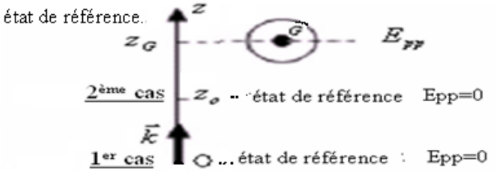
\includegraphics[width=0.5\textwidth]{./img/img00.png}
%\end{wrapfigure}
\section{Introduction : }
L’énergie cinétique et l’énergie potentielle ne sont pas les seules
formes d’énergie d’un système. Nous allons voir d’autres effets que
peut avoir le travail d’une force sur un système et ainsi on va
pouvoir définir une autre énergie qu’on appelle énergie interne.
Qu’est ce que l’énergie interne d’un système ?

\section{situation problème }
Le soleil transfert de l’énergie par rayonnement . lorsqu’on frotte
nous deux mains, l’une contre l’autre , elles s’échauffent. Les
hommes préhistorique ont réussi à faire des feu en frottant deux
morceaux de bois l’un contre l’autre . Dans tous ces exemples, il y
a élévation de la température.
Comment peut on expliquer cette élévation de la
température ?

\section{Quelques définitions : }

L’état macroscopique : 
L’état macroscopique de la matière concerne la matière qui est
accessibles à l’échelle humaine et en particulier dans la vie
quotidienne. Cet état est quantifié par la masse ou la quantité de
matière (g ou mol)

L’état microscopique :  de la matière concerne la matière à l’échelle
atomique ou moléculaire. Entre l’état macroscopique et
microcospique, il existe une constante de liaison : le nombre
d’Avogadro $N_A = 6,023×10^{23}$ particules par mole. Depuis les
années 80 grâce aux microscopes à effet tunnel et aux microscopes
à force atomique, on peut observer la surface des atomes.

NB : On a vu qu’une transfert d’énergie sous forme de travail peut
modifier l’énergie cinétique et/ou l’énergie potentielle de
pesanteur d’un corps solide.

\section{Effets du travail reçu par quelques systèmes:}
\subsection{Augmentation de la température : }
L'augmentation de la température, par les forces de frottement d'un frein, traduit une plus grande
agitation microscopique (donc une augmentation de l'énergie cinétique microscopique).

Exemple :lors de la découpe d'une plaque métallique a l'aide d'une meuleuse

En fournissant de l’énergie par travail à un système on peut élever sa température.

\subsection{ Changement d’état physique : }
\begin{wrapfigure}{r}{0.3\textwidth}
    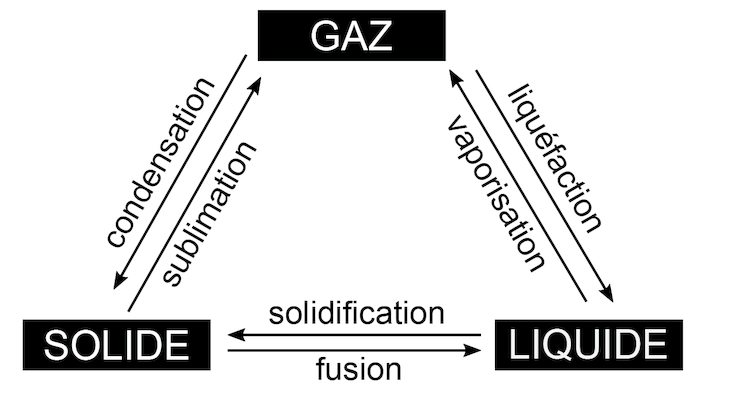
\includegraphics[width=0.3\textwidth]{./img/img01.jpg}
\end{wrapfigure}

Le travail des forces de frottement des skis sur la neige entraîne la fusion de la neige, donc une
modification des interactions microscopiques.

En fournissant de l’énergie par travail à un système on peut produire un changement d’état physique.

\subsection{Déformation élastique :}
Lorsqu'on tend un arc, il se déforme ce qui modifie les interactions microscopiques entre les
particules qui constituent l'arc Cette déformation de l'arc entraîne une mise en réserve d'énergie qui
pourra être cédée à la flèche.

En produisant des déformations de corps élastiques ceux-ci acquièrent.
une énergie qui sera stockée tant qu'ils restent déformés

\subsection{Augmentation de la pression d’un gaz : }
\subsubsection{Compression d’un gaz :  }
\begin{wrapfigure}{r}{0.2\textwidth}
    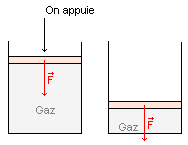
\includegraphics[width=0.2\textwidth]{./img/img02.png}
\end{wrapfigure}


Le travail de la force exercée par
l’expérimentateur a été utilisé pour
comprimer le gaz dont l’énergie
stockée augmente
\begin{wrapfigure}{r}{0.1\textwidth}
    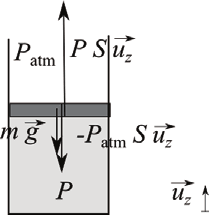
\includegraphics[width=0.1\textwidth]{./img/img03.png}
\end{wrapfigure}



\subsubsection{Travail de la force pressante: }


Lorsqu’une force n’est pas appliquée en un point mais répartie sur une surface, on dit
que la force est une force pressante
La pression P est le rapport de l'intensité de la force pressante F sur la surface de
contact S
$$P =\frac{F}{S} $$
Une force pressante produit sur la surface pressée un effet d’autant plus petit que l’aire de la
surface est grande.
$$W(F) = \vec{F}\vec{H} = F.H$$
avec $$F = P.S$$
A l'équilibre : $$F=P_f.S$$
Donc
$$W(F) = P_f.S(h_i - h_f) = P_f(V_i - V_f)$$

\subsubsection{Conclusion :}
Dans les exemples précédents, l'énergie reçue par le corps sous forme de travail à modifier
les interactions microscopiques entre les particules.

Comme à l'échelle macroscopique, on peut définir à l'échelle microscopique une énergie
cinétique due à l'agitation des particules et une énergie potentielle d'interaction due aux
positions des particules en interaction.

\section{Energie interne: }
\subsection{Définition :  }
L’énergie interne, notée U, d’un système est la somme des énergies cinétiques
microscopiques et des énergies potentielles d'interaction de toutes les particules du système
$$U = {E_C}_{mic} + {E_P}_{mic}$$

Remarque: On définit l’énergie totale E d’un système par
$$E = E_m + U  = E_c + E_{pp} + U$$
On ne peut pas calculer ${E_C}_{mic} + {E_P}_{mic}$ car la connaissance des vitesses et des
positions des particules est impossible du fait de leur nombre énorme.

\section{Echange d’énergie au cours d’une transformation :}
\subsection{Echange d’énergie :}
L’énergie peut s’échanger avec le milieu extérieur de deux manières différentes :

-Soit par échange de chaleur : Q (qui peut être reçue ou perdue le système).

-Soit par un travail :W , (qui peut être fourni ou reçu par le système).
\subsection{ Variation d’énergie d’un système :}
La variation d’énergie interne $\Delta$U d’un système résulte d’un échange d’énergie avec le milieu extérieur soit par un travail : W ou par un transfert de chaleur : Q
$$\Delta{U}=Q + W $$
avec $\Delta{U} =U_f - U_i$

S'il n'y a aucun échange de chaleur , $\Delta{Q}$ = 0 et donc $\Delta{U}$ = W. Dans ce cas , la variation d'énergie interne du système est égale au travail reçu ou fourni par le système.

Si aucun échange Travail n'est reçu ou fournit par le système , $W$ = 0 et donc $\Delta{U}$ = Q. Dans ce cas , la variation d'énergie interne du système est égale à la quantité de chaleur  échangee .

\subsection{Convention :}
En physique l’énergie transférée W, par travail au
système au cours d’une transformation (en joule),
est une grandeur algébrique :

W est positive W $>$ 0 si le système reçoit
effectivement l’énergie W.

W est  négative W $<$ 0 si le système fournit
effectivement l’énergie W.

\section{Premier principe de la thermodynamique : }
\subsection{Enoncé du 1er principe de la themodynamique:}
Au cours d'une transformation quelconque d'un système fermé, la variation de son énergie est égale à la quantité d'énergie échangée avec le milieu extérieur, par transfert thermique (chaleur) et transfert mécanique (travail).
$$\Delta{U}=Q + W $$

\subsection{transformation cyclique :}
Toute transformations qui amène le système de l’état initial à un état final identique à l’état initial est dite transformation
cyclique.$\Delta{U}= 0$
donc W = -Q le système reçoit l’énergie sous forme d’un travail et il la cède sous forme de chaleur ou inversement donc son énergie interne
ne subit aucune variation $U_f = U_i$
\subsection{Conséquence du premier principe :}
Pour un système isolé , c'est-à-dire un système qui n’échange aucune énergie avec le milieu extérieur , l’énergie totale
reste constante ,



\end{document}

